\section*{Results and Discussion}

%%%%%%%%%%%%%%%%%%%%%%%%%%%%%%%%%%%%%%%%%%%%%%%%%%%%%%%%%%%%
\renewcommand{\arraystretch}{1.1}
\begin{table}[tb]

\begin{center}
 \caption[]{Silent site $F_{ST}$ from GBS SNPs \hspace*{2.3cm}}
  \textbf{}\\[-2mm]
{\fontsize{7}{9}\sf
    \begin{tabular}{llccccccl}
    \hline
    & & \\[-3mm]
	&		&	\multicolumn{2}{c}{Mexico}		&	\multicolumn{2}{c}{South America}		\\
	&		&	Lowlands	&	Highlands	&	Lowlands	&	Highlands	\\
      \hline
    & & \\[-3mm]
Mexico	&	Lowlands	&	--	&		&		&		\\
	&	Highlands	&	0.0244	&	--	&		&		\\
SA	&	Lowlands	&	0.0227	&	0.0343	&	--	&		\\
	&	Highlands	&	0.0466	&	0.0534	&	0.0442	&	--	\\ [1mm]
    \hline
    \end{tabular}
    \label{FstP}  % caption is needed to make this work
}
\end{center}
\end{table}
\renewcommand{\arraystretch}{1}
%%%%%%%%%%%%%%%%%%%%%%%%%%%%%%%%%%%%%%%%%%%%%%%%%%%%%%%%%%%%

%Matt, please add a sentence or two at the start say "we sampled X, genotyped using Y etc.?? You can use stats from the paragraph below on total number of SNPs
%MBH: So this is already in the Methods.  Do we need to recapitulate here?
%Yes, think so. For PLOS, results goes before methods. A brief summary so someone has a basic idea what we did. If you don't think it's needed, I can be convinced otherwise.
%Sho, please move some of the other numbers below (SNPs tested etc.) to methods.
%
%\subsubsection{Joint data set}In total, 91,779 SNPs remained in our joint, filtered GBS and MaizeSNP50 data set ($2n\geq20$ and HWE $P\geq0.005$ \mbh{need to keep track of how this is reported: sometimes 0.005, sometimes 0.5\%} for GBS or $P\geq0.05$ for MaizeSNP50 for all four populations).  For the Mexican and South American populations, we calculated $P$-values for 76,989 and 63,160 SNPs respectively with the remaining SNPs being monomorphic. The reduced number of polymorphic SNPs in South America relative to Mexico is likely due to a lower effective population size in the South American populations.  48,370 SNPs were polymorphic in both Mexico and South America. 

\subsection*{Population structure}

We performed a {\sf STRUCTURE} analysis \citep{Pritchard_2000_10835412,Falush_2003_12930761} of our landrace sample, varying the number of groups from $K=2\sim 6$ (Figure \ref{map}, Supp FigX). 
%cite supp. figure with likelihood plot from STRUCTURE
Most landraces were assigned to groups consistent with \emph{a priori} population definitions, but admixture between highland and lowland populations was evident at intermediate elevations ($\sim1700$m).  Consistent with previously described scenarios for maize diffusion \citep{Piperno_2006_69}, we find evidence of shared ancestry between lowland Mexican maize and both Mexican highland and South American lowland populations.  Pairwise $F_{ST}$ among populations reveals low overall differentiation (Table~\ref{FstP}), and the higher $F_{ST}$ values observed in South America are consistent with decreased admixture seen in STRUCTURE.  Archaeological evidence supports a more recent colonization of the highlands in South America  \citep{Piperno_2006_69,Perry_2006_16511492,Grobman_2012_22307642}, suggesting that the observed differentiation may be the result of a stronger  bottleneck during colonization of the South American highlands. 

\subsection*{Population differentiation under inferred demography}

To provide a null expectation for allele frequency differentiation, we used the joint site frequency distribution (JFD) of lowland and highland populations to estimate parameters of two demographic models (Fig.~\ref{model}) using the maximum likelihood method implemented in {\sf dadi} \citep{Gutenkunst_2009_19851460}.  
Estimated parameter values are listed in Table~\ref{param}; 
while the observed and expected JFDs were quite similar for both models,  
residuals indicated an excess of rare variants in the observed JFDs in all cases (Fig.~\ref{JFD}). 
Under both models IA and IB,  we found expansion in the highland population in Mexico to be unlikely, but a strong bottleneck followed by population expansion is supported in South American maize in both models IA and II.  
The likelihood value of model IB was higher than the likelihood of model IA by 850 units of log-likelihood (Table~\ref{param}), 
consistent with analyses suggesting that introgression from \textit{mexicana} played a significant role during the spread of maize into the Mexican highlands \citep{Profford_2013}. 

In addition to the parameters listed in Fig.~\ref{model}, we investigated the impact of varying the domestication bottleneck size ($N_B$).  
Surprisingly, $N_B$ was estimated to be equal to $N_C$, the population size at the end of the bottleneck, and the likelihood of $N_B<N_C$ was much smaller than for alternative parameterizations (Table~\ref{param}, supp table~3) 
%please go through and check we have these supp. tables and they are cited in the correct order.
This result appears to contradict earlier work using sequences from coding regions to infer a maize domestication bottleneck \citep{Wright_2005_15919994, Tenaillon2004}.  One explanation for this discrepancy may be the action of purifying selection in coding regions, which could act to retard the recovery of diversity and lead to estimates of a stronger bottleneck \citep{Hufford_2012_22660546}.  Consistent with \citet{Hufford_2012_22660546}, our genome-wide SNP data show an excess of rare variants relative to expectations under \citet{Wright_2005_15919994}'s bottleneck model (Fig.~\ref{JFD}), suggesting a domestication model involving a weaker bottleneck or more rapid population growth.
% Peter does more rapid pop growth make sense? I don't think it's really more rapid, I think it's just that the lack of rare variants in coding regions leads to over-estimation of bneck strength. Is that plausible (graham seemed skeptical when I mentioned this).

Comparing our empirical $F_{ST}$ values to the null expectation simulated under our demographic models allowed us to identify significantly differentiated SNPs between low- and highland populations. In all cases, observed $F_{ST}$ values were quite similar to those generated under our null models  (Figure~\ref{FstDist}A), and model choice -- including the parameterization of the domestication bottleneck -- had little impact on the distribution of estimated of p-values (Supp Figure~4). We chose $P<0.01$ as an arbitrary cut-off for significant differentiation between low- and highland populations, and identified 1,040 SNPs in Mexico (1,040/76,989=0.0135) and 756 SNPs in South America (756/63,160=0.0120) as outliers.  

%%%%%%%%%%%%%%%%%%%%%%%%%%%%%%%%%%%%%%%%%% FIGURE
\begin{figure}[tb]   
  \begin{center}
   \vspace{-0mm}
   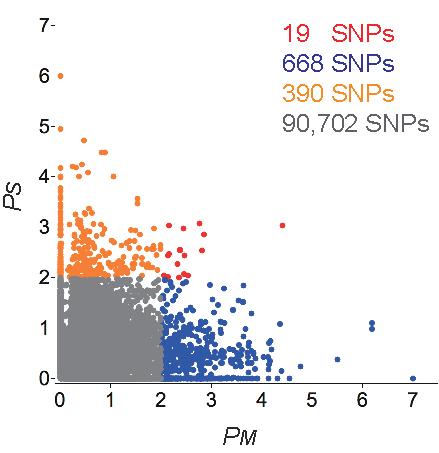
\includegraphics[width=0.4\textwidth]{fig/Fig6}
   \renewcommand{\baselinestretch}{0.9}
   \vspace{-3mm}
   \caption{Scatter plot of $F_{ST}$ $P$-values in Mexico ($P_M$ on $x$-axes) and South America ($P_S$ on $y$-axes).  $P_M$ and $P_S$ are scaled by $-\log_{10}$.  
   \plr{I think you mean these are $-\log_{10} P$-values?}
   \plr{It might be nice to label this figure with the numbers in the text, so we can see how many SNPs fall in each category.}
   Red, blue, orange and gray dots represents SNPs showing significance in both Mexico and South America, only in Mexico, only in South America, respectively (see text for details).} 
\vspace{-6mm}
    \label{PvDist}
  \end{center}
\end{figure}
%%%%%%%%%%%%%%%%%%%%%%%%%%%%%%%%%%%%%%%%%% FIGURE
%
%do we know what that clear outlier red SNP is? anything interesting?

\subsection*{Patterns of adaptation}

\subsubsection{Adaptation via mutation versus standing variation}

In order to characterize patterns of adaptation, we first determined whether  SNPs showing high differentiation between the lowlands and the highlands arose primarily through new mutations or standing genetic variation.  
We found that these putatively adaptive variants in both Mexico and South America tended to segregate in lowland populations more often than other SNPs (84.6\% vs. 74.8\% in Mexico, $P < 10^{-11}$ by Fisher's exact test (FET) and 87.3\% vs 81.8\% in South America,  $P< 10^{-3}$).  
\plr{``segregate in'' -- are these percentages of SNPs that are polymorphic (as opposed to fixed for either allele) in the relevant population?}
We extended this analysis to standing variation in \textit{parviglumis} by retrieving SNP data from 14 \textit{parviglumis} inbred lines included in the Hapmap v2 data set, using only SNPs with $n\geq10$ \citep{Hufford_2012_22660546}.  Again we found that putatively adaptive variants were more likely to be polymorphic in \textit{parviglumis} (81.1\% vs. 72.1\% in Mexico, FET {$P < 10^{-6}$ and 81.2\% vs 72.7\% in South America,  $P< 10^{-4}$).  
%MBH: Sho, I extensively edited the previous sentences of this paragraph.  I was careful to keep all \%'s and $P$-values straight, but might be a good idea to double check

These results suggest that maize adaptation to high altitudes has largely made use of standing genetic variation. 
%etc.evidence for selection from standing variation is increased in model organisms such as Drosophila (Petrov arXiv) and human \citep{Turchin_2012_22902787,Peter_2012_23071458}.}
%Sho: please add a sentence or two here on other empirical results on standing var (including the above). We also need a sentence or two here on why we expect this based on theory. I think we drop the domestication comparison
Because linkage disequilibrium in maize decays rapidly (CITE), it is plausible that a number of hard sweeps -- strong selection on new mutations -- would be missed by our data, but several lines of evidence suggest to us that this is unlikely.  
%Guys, help here.  My thinking is:
% 1) we see few private SNPs (true? I didn't quite understand your email Sho. what % of SNPs are unique to a population when we include teosinte?
% 2) We do see evidence of selection on other SNPs (at least high Fst), suggesting that even if there are hard sweeps we missed, a substantial amount of selection on standing var appears to have occurred.
% 3) The number of hard sweeps couldn't have been huge or we would see some.
% We need to summarize whether we believe the missed hard sweeps idea is likely or not in a few sentences. Sho, what do you think? Take a stab at it?

\subsubsection{Highland versus lowland adaptation}  

Given the historical spread of maize from an origin in the lowlands, it is tempting to assume that significant population differentiation should be primarily due to an increase in frequency of adaptive alleles in the highlands.
To test this hypothesis, we sought to identify the adaptive allele at each locus using comparisons between Mexico and South America as well as to \emph{parviglumis} (Supplemental methods).
%
%I think these bar graphs and explanation should go in the supplement. Opinions?
%MBH:I think the edits below improve the narrative, but they gut the results; it makes it easy on the reader that just wants to trust us on the details, but personally I would want more details before I'd buy these results and then I'd be annoyed that I had to dig through the supplement in order to get them.
%
%However, we cannot rule out the possibility of adaptation in the lowlands.
%Therefore we further investigated patterns of allele frequency change across populations.
%When data were available for \textit{parviglumis} from Hapmap v2 \citep{Chia_2012_22660545,Hufford_2012_22660546}, we included these in our analysis.
%
%First, we assessed patterns of allele frequencies in SNPs that were significantly differentiated between highland and lowland maize.
%We focused on SNPs segregating as shown in Fig.~\ref{tes2}A, although some SNPs showed more complex patterns.
%The first and second rows show hypothesized patterns of segregation under highland adaptation; here, allele frequencies in maize from a highland region are highly differentiated from those of \textit{parviglumis} and maize from the corresponding lowland region. %and no difference is observed between South America populations.
%When \textit{parviglumis} data are lacking, SNPs showing the pattern of segregation in the third row likely underly highland adaptation.
%\mbh{don't think this row in the figure is necessary}
%Similarly, patterns of SNP segregation depicted in the fourth to sixth rows are consistent with lowland adaptation.
%The patterns expected for highland and lowland adaptation in South America are qualitatively the same as those shown for Mexico in Fig.~\ref{tes2}A.
%
Consistent with predictions, we infer that differentiation at X\% (537) and Y\% (530) of SNPs in Mexico and South America is due to adaptation in the highlands, with only A\% and B\% of SNPs inferred to be due to lowland adaptation. The majority of these SNPs show patterns of haplotype variation consistent with our inference (Supp. Table X).
%This supp. table should show numbers and % of PHS stats and allele segregation patterns. Easier to parse in a table.
%
%inferred to be adapted in highland or lowland environments showe(74.5\% in Mexico and 84.5\% in South America) of putatively highland-adaptive SNPs also had lower P-values for the PHS test in highland maize. 
%Likewise, 63.5\% and 67.1\% of the putatively adaptive SNPs in Mexico and South America that showed segregation patterns consistent with lowland adaptation also showed lower P-values for the PHS test in lowland maize.
%Additionally, when a putatively derived allele segregated in both the lowlands and highlands but was more prevalent in the highlands, 67.5\% and 67.6\% of such SNPs showed lower PHS $P$-values in the highlands in Mexico and South America. 
%\comst{I tested: $P<10^{-11}, < 0.01$, $\approx 0$, $<10^{-9}$ for Mex high, Mex low, SA high and SA low, respectively}

\subsubsection{Adaptation through introgression}

A marked difference between highland adaptation of maize in Mexico and South America is the potential for adaptation through introgression from wild relatives.  While maize in Mexico grows in sympatry with both the lowland taxon \textit{parviglumis} and the highland taxon \textit{mexicana}, maize in South America is outside the range of wild \textit{Zea} species.
 \citep{Pyhajarvi2013} recently assessed the potential for local adaptation in \textit{parviglumis} and \textit{mexicana} populations, characterizing differentiation between these subspecies using an Fst-outlier approach.
We observed a significant excess of overlap between our putatively adaptive SNPs in Mexican maize and those identified in the \citep{Pyhajarvi2013} analysis (Table~\ref{tanja}; $P<0.01$ by FET). Similar to that paper, we also find that SNPs with significant $F_{ST}$ $P$-values are enriched in intergenic regions compared to non-sigificiant SNPs (51.3\% vs. 44.2\%; FET $P < 10^{-8}$). Significant overlap was also observed between signficant SNPs in South America and teosinte ($P<0.01$), but the proportion of SNPs was lower than observed in Mexico.  These data suggest that adaptations in Mexican maize may have been obtained through gene flow with wild relatives.  To more fully explore this hypothesis we evaluated our data in light of introgression identified by \citep{Profford_2013} from \textit{mexicana} into maize in the Mexico highlands.  
The proportion of significant SNPs in introgressed regions in Mexico is significantly higher than found in South America (FET $P\ll0.001$).
%When focusing on GUs, we identified 99/586 (14.5\%) and 22/466 (4.7\%) GUs of Mexico- and SA-specific significance in introgressed regions (Fisher's exact test, $P<10^{-6}$). 
%Would the genetic unit numbers work in the tanja table? i liek those numbers and think we should keep if possible.
Outside introgressed regions, the Mexican and South American populations did not show marked differences in the proportion of significant SNPs (Fisher's exact test, $P>0.7$). These results add to those of \citep{Profford_2013}, suggesting that SNPs in the introgressed regions identified have indeed been under selection.  

\subsubsection{Evidence for parallel adaptation}
\plr{Should be ``No evidence for\ldots''?}

While maize adaptation in Mexico and South America are likely distinguished by unique histories of gene flow with wild relatives, the potential remains for parallel adaptation in these two regions.  
SNPs showing significant differentiation between low- and highland populations in both Mexico and South America are likely candidates for parallel adaptation. 
We identify 56 SNPs with $F_{ST}$ p-values in Mexico ($P_M$) and South America ($P_S$) both $<0.01$.   
This number  was significantly larger than the random expectation ($48,370\times 0.01 \times 0.01 \approx 4.8$; $\chi^2$-test, $P\ll0.001$).  Furthermore, the distribution of $P_M$ in the 712 SNPs with $P_S<0.01$ was highly skewed toward zero (supp fig~7A), and a similar tendency was observed in $P_S$ given $P_M<0.01$ (935 SNPs; supp fig~7B).  Thus, we converted the $P$-values in one population given $P<0.01$ in the other population into $q$-values.  
At a false discovery rate of 0.2 we found 117 SNPs with $P_M<0.01 \cap P_S < 0.0169$ or $P_M<0.0247 \cap P_S < 0.01$, and these SNPs were considered our candidates for parallel adaptation.
We found 959 SNPs showing significant population differentiation only in Mexico ($P_M<0.01 \cap P_S > 0.0169$) and 664 SNPs only in South America  ($P_M>0.0247 \cap P_S < 0.01$).  The scatter plot of $P_M$ and $P_S$ is shown in Figure~\ref{PvDist}.  
For a subset of 67 of the SNPs showing putative evidence of parallel adaptation candidates we also had data from \textit{parviglumis} and were able to infer based on patterns of segregation whether these SNPs were potentially adaptive under lowland or highland conditions.  Surprisingly, SNPs identified as targets of parallel adaptation in Mexico and South America more frequently show segregation patterns consistent with lowland adaptation (62 SNPs) than highland adaptation (5 SNPs). %add p-value for this comparison?
%70\% and 39.5\% of SNPs showed consistent patterns in the PHS tests in high- and lowland populations, respectively.
%Not sure what these PHS values are referring to? Do we need to keep them?
%
%Without data from \textit{parviglumis}, it is very difficult to decipher whether a segregation pattern is consistent with high- or lowland parallel adaptation.  
%\st{In total, 1,740 SNPs showed the signature of selection both or either in Mexico and South America} \
%
%Can we just skip the above commented-out text?
%
In addition to evaluating parallel adaptation at the SNP level, we investigated how often different SNPs in the same gene may have been targeted by selection. To search for this pattern, we define a "genetic unit" or GU as all SNPs within 10kb of a transcript.  SNPs in an miRNA or second transcript within 10kb of the transcript of interest were excluded.  
We classified SNPs showing significance in Mexico, South America or in both regions into 1,277 GUs. 
Of these, 95 GUs contained at least one SNP with a pattern of differentiation suggesting parallel adaptation, whereas only 12 GUs contained both Mexico-specific and SA-specific significant SNPs. 
%I don't understand what these 95 show. 1 significant and one nonsignficiant SNP? whereas the 12 are significant in both?
%MBH:  So I was assuming this meant that 95 GUs had a SNP with the same allele at high frequency in the highlands of both SA and Mexico (not significant in both but still consistent with parallel adaptation) and 12 of these had one SNP in a GU significant in Mexico and another in the same GU significant in South America (also parallel adaptation if you assume the SNPs result in the same phenotype); needs some clarification!
Overall, fewer GUs showed evidence of parallel adaptation than expected by chance ($P<10^{-5}$), with more than 700 and 470 GUs showing Mexico-specific and SA-specific significant SNPs, respectively.  
Despite similar phenotypes and environments, we thus see little evidence for parallel adaptation at either the SNP or the gene (GU) level.  
This contrasts with data from humans \citep{Tennessen_2011_21698142} showing frequent evidence of selection on the same genes in multiple pairs of tropical and temperate human populations.  
%Points for discussion (add/delete etc.)
%genomic architecture differences? local adaptation uses regulary in teo (cite Tanja)? But what about Fraser (finds same in humans)
% More likely: target size

%perhaps below should be moved to methods or supp? seems out of place here.
%First, we randomly picked 959 and 664 SNPs that represent Mexico- and SA-specific differentiation (see above) from 91,779 positions and counted the number of GUs under Pattern C.

%this needs to ve moved
%CUTME
%While some have hypothesized that pre-adapted highland maize was transported through Central America to the Andes based on analysis of the \emph{Adh2} locus \citep{Freitas_2003_68}, analysis of larger sets of molecular markers suggests \emph{de novo} highland adaptation in South America \citep{Vigouroux_2008_21632329,vanHeerwaarden_2011_21189301}.  Our result of rare parallel adaptation may be consistent with independent origins of highland populations, not gene flow between the two highland populations.
%MBH:Like the discussion above...any way we could include this somewhere?

%Fig.~\ref{tes2}B shows the segregation patterns expected under parallel adaptation in the highlands and the lowlands.
%If there is not teosinte data, we cannot distinguish between high- and lowland adaptation.
%Surprisingly, SNPs identified as targets of parallel adaptation in Mexico and South America more frequently show segregation patterns consistent with lowland adaptation (62 SNPs) than highland adaptation (5 SNPs).
%70\% and 39.5\% of SNPs showed consistent patterns in the PHS tests in high- and lowland populations, respectively.

%Without data from \textit{parviglumis}, it is very difficult to decipher whether a segregation pattern is consistent with high- or lowland parallel adaptation.  

\subsection*{Comparison to theory}

% # \mutrate computation:
% A <- 500; rho <- 5000; sb <- 10^(-(1:4)); xisq <- 30
% sapply( 10^c(-5,-8), function (mu) mu * (2 * rho * A * sb)/xisq )

For a final point of comparison,
we assessed the degree of parallelism expected under a spatially explicit population genetic model.
We estimate the (maize) population density $\rho$ of the highlands to be around
(0.5 people/km$^2$) $\times$ (0.5 ha field/person) $\times$ ($2\times10^4$ plants per field ha) $=$ 5,000 plants per km$^2$.
The area of the Andean highlands is around $A=500\text{km}^2$, leading to a total population of $A \rho = 2.5 \times 10^6$.
%MBH: This seems like a pretty low planting density
%This should be 14K plants per acre, or ~30-35K per hectare. Good catch Matt!!
%  Moved this up here.  I'm not sure what that 14,000 number was doing in the previous draft.  But, added details behind this calculation.  Should I change anything?
%  Note that 0.5 people/km2 is close to the other number we came up with of "one village per 15km" (which gets 0.4444 people/km2).
Combined with an offspring variance of $\xi^2 = 30$,
we can compute the rate $\mutrate$ at which newly adapted alleles arise in the population.
We observe that even if there is strong selection for an allele at high elevation ($s_b=0.1$),
a single-base mutation with mutation rate $\mu=10^{-8}$ would still take at least 6,000 generations to appear and fix.
On the other hand, a kilobase-sized target with mutation rate $\mu=10^{-5}$
with this selection coefficient would appear and begin to fix in only 6 generations,
while more weakly selected alleles with $s_b$ of $10^{-2}$ or $10^{-3}$ would take hundreds or thousands of generations, respectively.
(Note that the time scales linearly with the selection coefficient: at these values $\Tmut = 1/\mutrate \approx \mu s_b \times 1.6\times 10^5$.)
Therefore, we might expect to see parallel changes of similar effect at the level of genes (e.g.\ disabling mutations),
but would not expect to see adaptive SNPs that arise through independent mutation in the two populations.

% # Tmig computation:
% A <- 500; rho <- 5000; sm <- 10^(-(1:4)); xisq <- 30; sigma <- 1.8
% 1/(sqrt(2*sm)/sigma)
% sapply( 1000*(1:4), function (R) 1 / ( A * rho * ( sqrt(2*sm) / xisq ) * exp(- sqrt(2*sm)*R/sigma ) ) )
% Ne <- (561/10^5)*A*rho 
% Ne  # = 14025
% sapply( 1000*(1:4), function (R) 1 / ( Ne * exp(- sqrt(2*sm)*R/sigma ) ) )

Parallel SNP changes seem unlikely from new mutation; 
what about gene flow between the highlands?
From the demographic model above
we have estimated that $\sigma \approx 1.8$ kilometers per generation,
so with $10^{-1} \ge s_m \ge 10^{-4}$ the distance $\sigma/\sqrt{2s_m}$ over which the frequency of 
a highland-adaptive, lowland-deleterious allele decays into the lowlands
is still short: between 4 and 150 kilometers.
Since the Mexican and Andean highlands are around 4,000 km apart,
the time needed for a rare allele, with selective cost $s_m=10^{-3}$ in the lowlands, to transit between the two highlands
is $\Tmig \approx 5 \times 10^{34}$ generations.
In other words, from these calculations it is almost impossible that an allele that is deleterious at low elevation with $s_m=10^{-3}$ 
would ever transit from the Mexican to the Andean highlands.
If the selection against the allele is even weaker ($s_m=10^{-4}$) it is still expected to take $\Tmig = 1.8 \times 10^8$ generations.
However, shorter distances could be transited by very weakly deleterious alleles --
if the distance between highland patches $R$ is 1,000 km (or if $\sigma$ is four times larger)
then with $s_m=10^{-4}$ the time $\Tmig$ is about 1.6 generations --
so, adaptation by migration is certain.
This is strongly dependent on the small value of the deleterious selection coefficient: 
with even $s_m=10^{-3}$ it is still $2.3 \times 10^6$ generations.

This suggests that if the highland-adaptive mutations are even weakly deleterious in the lowlands,
gene flow will not result in shared adaptations.
The situation where they are neutral in the lowlands is harder to model,
but we can make some informed guesses.
Maize in the Andean highlands, say, would have inherited a neutral, highland-adapted allele from the Mexican highlands 
if some of the ancestral lineages along which the modern Andean plants have inherited at that locus trace back to the Mexican highlands 
at some point since the appearance of the allele in Mexico.
If the allele is neutral in the lowlands, we can treat this as a neutral process,
using the framework of coalescent theory \citep{wakeley2005coalescent}.
To do this, we need to follow \emph{all} of the $N \approx 2.5 \times 10^6$ lineages backwards --
but, these quickly coalesce to many fewer -- to $m$ lineages
in approximately $\sum_{k=m}^N \frac{2N}{\xi^2 k(k+1)} \approx 1.25 \times 10^5/m$ generations;
leaving about 1000 lineages after 100 generations.
These lineages are starting to be spread out over a larger area.
The displacement of a lineage after $m$ generations has variance $m \sigma^2$ and perhaps approximately Gaussian;
if we assume that $n$ of them are independent, and $Z_n$ is the distance to the furthest one,
then $\P\{ Z_n / \sqrt{m \sigma^2} \le x /\sqrt{2 \log n} + \sqrt{2 \log n} - (1/2) (\log \log n + \log 4 \pi)/\sqrt{2 \log n} \} \approx \exp( - e^{-x} )$
\citep{berman1964limit}.
With $n=1000$, the typical distance to the furthest displacement is after $m=1000$ generations is $\sqrt{2 \sigma^2 m \log n} 212$km;
after $m=6000$ generations it is $\approx 518$km.
In either case the chance that the maximum is larger than even 1,000km after 6,000 generations is well less than $10^{-4}$.
Of course, this is under an equilibrium population model; and maize reached the Andean highlands only around 4,000 years ago.
Nonetheless, this suggests that even highland-adapted allele that are merely neutral in the lowlands
would have difficulty moving between the Andean and Mexican highlands in a few thousand generations.

In conclusion, population genetics theory suggests that
parallel adaptation involving identical nucleotide changes is quite unlikely under either scenarios of independent mutation 
or transit of central America by undirected (diffusive) sharing of seed.
However, independent mutations could be expected in kilobase-size targets,
suggesting there might be signal for genes that share adaptive changes.
The conclusions could change if we drastically underestimate the rate of very long distance sharing of seed,
e.g.\ if sharing across hundreds of kilometers was common at some point.

